\documentclass{beamer}

\usetheme[]{Rochester}
\usecolortheme{beaver}
\usepackage[latin1]{inputenc}
\usepackage{graphics}

\author{Will Webberley}
\date{Autumn 2014}
\institute[COMSC]{Cardiff School of Computer Science and Informatics}



\title{System-Specific Design}
\subtitle{CM2101: Human-Computer Interaction}

\begin{document}

\frame{\titlepage}

\frame{
    \frametitle{System-specific design}
    \begin{itemize}
        \item Important for ensuring consistency within a platform (`semi-external' consistency)
        \item Use the controls, layout, functions common to that platform
        \item Ensures compatibility with platform
    \end{itemize}
}

\frame{
    \frametitle{System-specific design}
    \textbf{Advantages}
    \begin{itemize}
        \item Address learnability
        \begin{itemize}
            \item Predictability (user knows what to expect)
            \item Familiarity (controls and visualisations more familiar to the user)
            \item Generalisability (if can use one app on iOS, others should be easier to learn)
        \end{itemize}
        \item Address consistency
        \item Address recognition vs. recall
        \item Often faster when native
        \item Survivability/modernisation after OS updates
    \end{itemize}
}

\frame{
    \frametitle{System-specific design}
    \textbf{Disadvantages}
    \begin{itemize}
        \item Might be completely different design between platforms
        \item Require a team for each platform
        \item Entirely distinct codebases
        \item Entirely distinct development cycle (i.e. own design-implementation-evaluation cycle)
        \item Requires a mix of expertise (more expensive)
        \item If not enough time/money/expertise, you become limited by the platforms you \textit{can} develop for 
    \end{itemize}
    Many of these explain the move to HTML5/JS mobile apps (e.g. using Cordova/PhoneGap):
    \begin{itemize}
        \item One codebase (mostly)
        \item One development cycle
        \item One team
        \item Still multiple test stages, however
    \end{itemize}
}

\frame{
    \frametitle{Designing for iOS}  
    Human interface guidelines: \\
    \begin{footnotesize}developer.apple.com/library/ios/documentation/userexperience/conceptual/mobilehig\end{footnotesize}
    \vskip20pt
    \begin{columns}
        \column{.8\textwidth}
            \textbf{iOS designed to embody:}
            \begin{itemize}
                \item \alert{Deference} - UI helps people understand content
                \item \alert{Clarity} - Text legible, icons sensible and precise
                \item \alert{Depth} - Use of visual layers, `heighten people's delight and understanding'
            \end{itemize}
            \vskip20pt
        \column{.2\textwidth}
            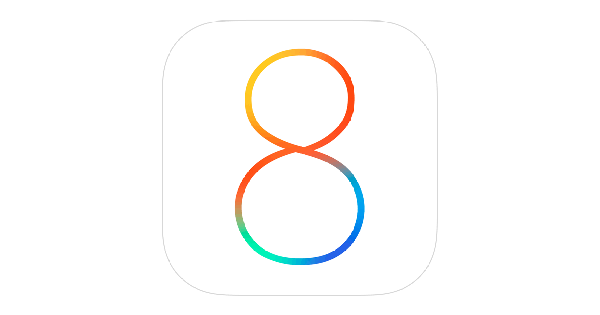
\includegraphics[width=2cm]{media/ios8.png}
    \end{columns}        
    iOS clearly focussing on \alert{Learnability} and \alert{Satisfaction}.
}

\frame{
    \frametitle{iOS: Design principles}
    \begin{columns}
        \column{.5\textwidth}
            \begin{itemize}
                \item Aesthetic integrity
                \begin{itemize}
                    \item How well an app's appearance integrates with its function
                \end{itemize}
                \item Consistency
                \begin{itemize}
                    \item Transfer knowledge from one iOS app to another
                    \item Clear link to \alert{Generalisability}
                \end{itemize}
                                \item Feedback
                \begin{itemize}
                    \item Acknowledge actions, show results and progress
                \end{itemize}
            \end{itemize}
        \column{.5\textwidth}
            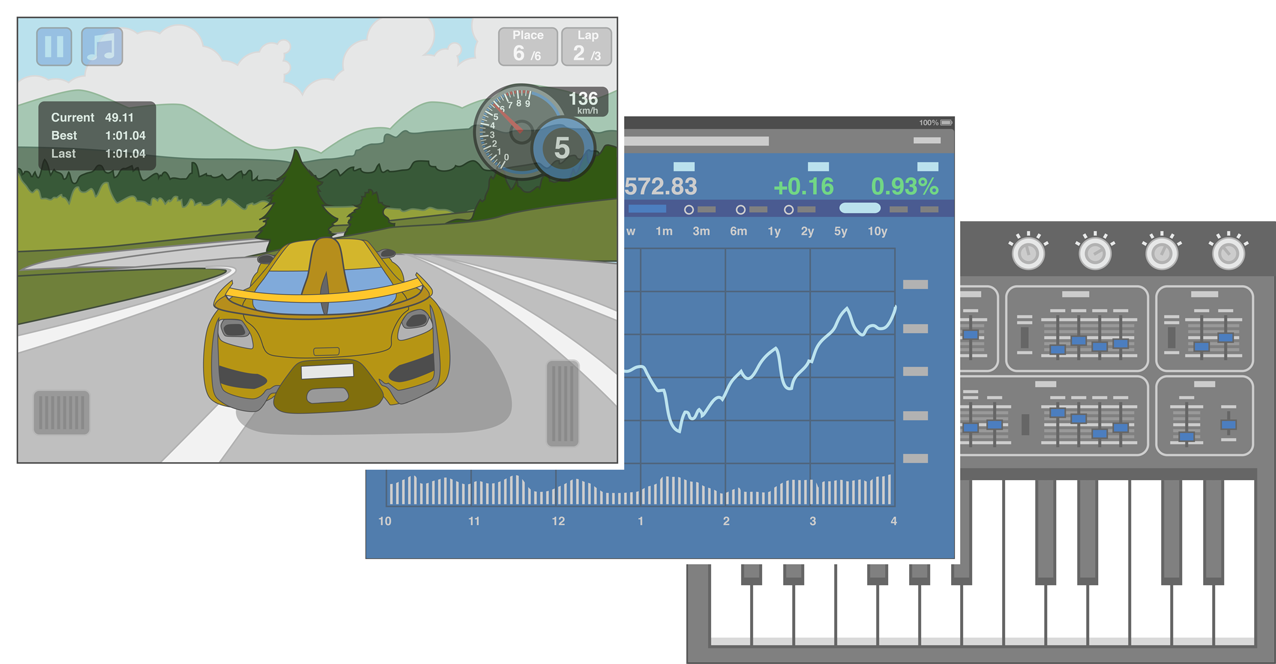
\includegraphics[width=5cm]{media/integrity.png}
    \end{columns}
}

\frame{
    \frametitle{iOS: Design principles}
    \begin{columns}
        \column{.5\textwidth}
            \begin{itemize}
                \item Direct manipulation
                \begin{itemize}
                    \item People directly manipulate onscreen objects instead of other controls
                    \item Clear link to \alert{Mapping} and \alert{Affordance}
                \end{itemize}
                \item Metaphors
                \begin{itemize}
                    \item Objects and actopns metaphors for familiar experiences
                    \item Linked to \alert{Mapping} and \alert{Familiarity}
                \end{itemize}
                \item User control
                \begin{itemize}
                    \item People should start actions, let people make decisions
                    \item \alert{User Control} general principle
                \end{itemize}
            \end{itemize}
        \column{.5\textwidth}
            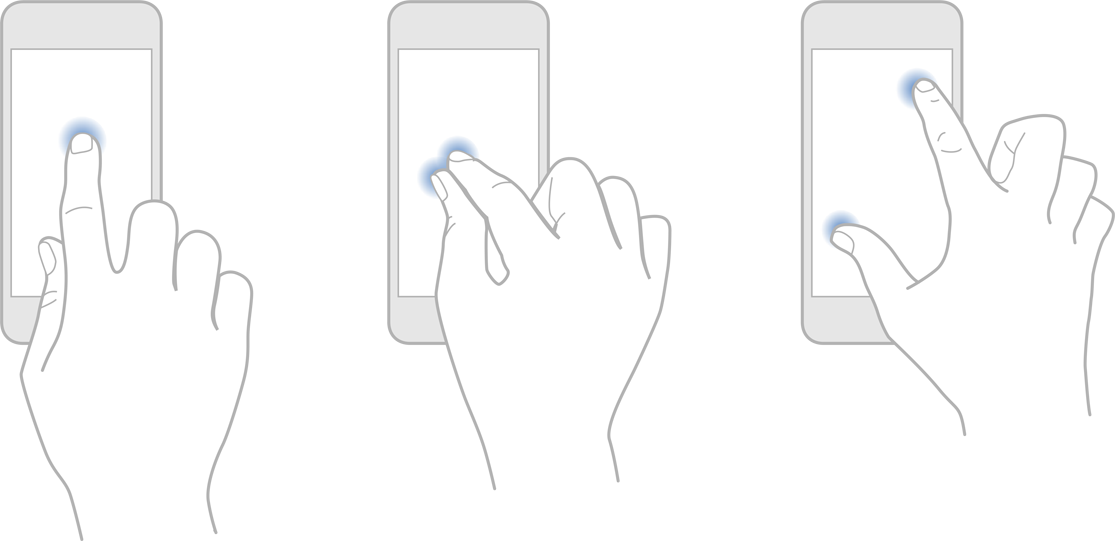
\includegraphics[width=5cm]{media/manipulation.png}
    \end{columns}
}

\frame{
    \frametitle{iOS: App anatomy}
    \textbf{Four main UI element types: \alert{bars}, \alert{content views}, \alert{controls}, \alert{temporary views}}
    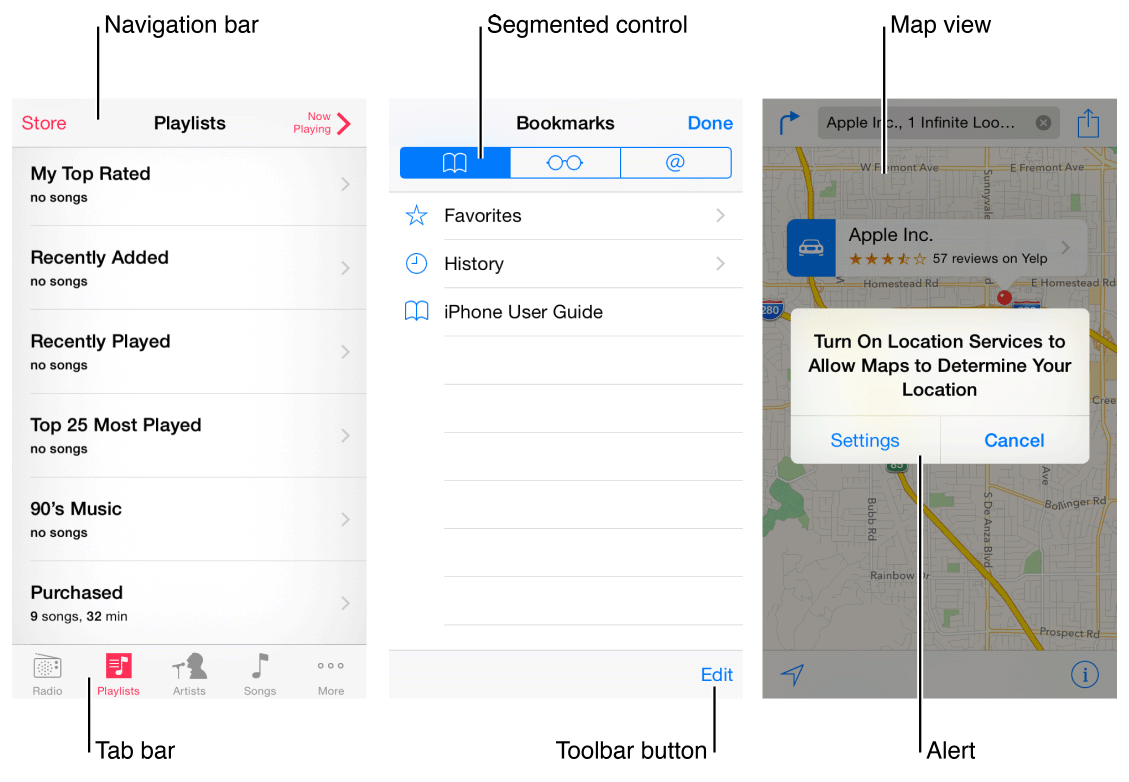
\includegraphics[width=.8\textwidth]{media/anatomy.png}
}

\frame{
    \frametitle{iOS: Layout guidelines}
    \begin{columns}
        \column{.5\textwidth}
            \textbf{Task focus}
            \vskip10pt
            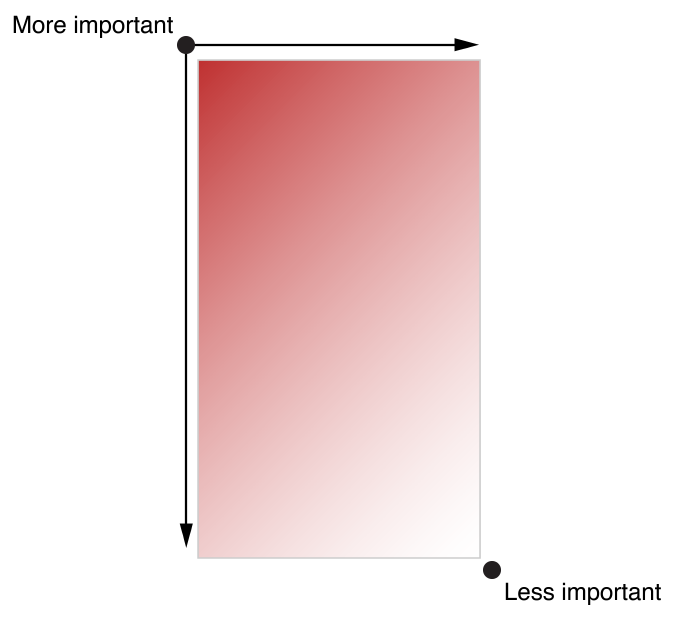
\includegraphics[width=6cm]{media/focus.png}
        \column{.5\textwidth}
            \textbf{Visual weight}
            \vskip10pt
            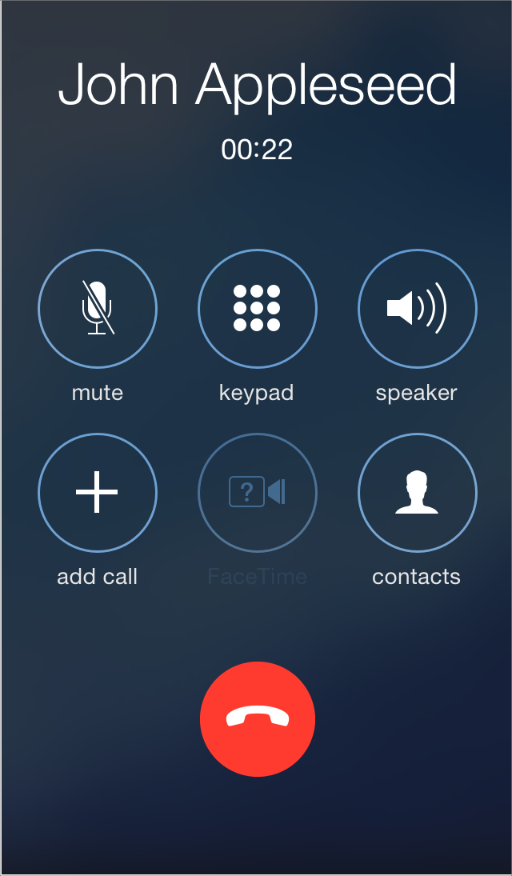
\includegraphics[width=4cm]{media/weight.png}
    \end{columns}
}

\frame{
    \frametitle{iOS: Starting apps}
    Apps should:
    \begin{itemize}
        \item Start instantly
        \item Avoid \textbf{splash screens} 
        \item \textbf{Delay login requirement} for as long as possible
        \item Launch in \textbf{current orientation}
        \item Restore from previous state, if available
        \item Avoid disclaimers or license agreements before user can do anything else
    \end{itemize}
}

\frame{
    \frametitle{iOS: Starting apps}
    \begin{columns}
        \column{.5\textwidth}
            \textbf{Good}
            \vskip5pt
            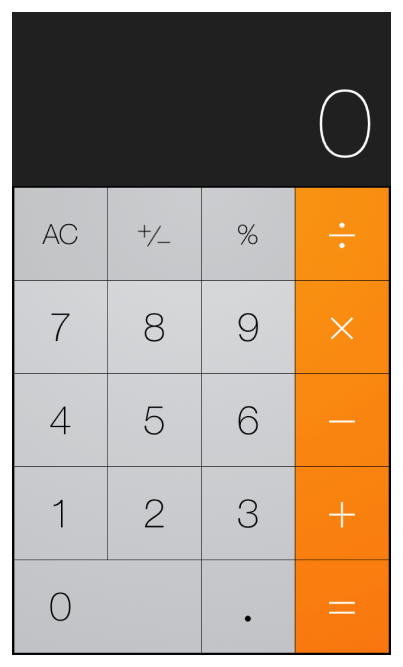
\includegraphics[width=4cm]{media/starting_1.png}
        \column{.5\textwidth}
            \textbf{Bad}
            \vskip5pt
            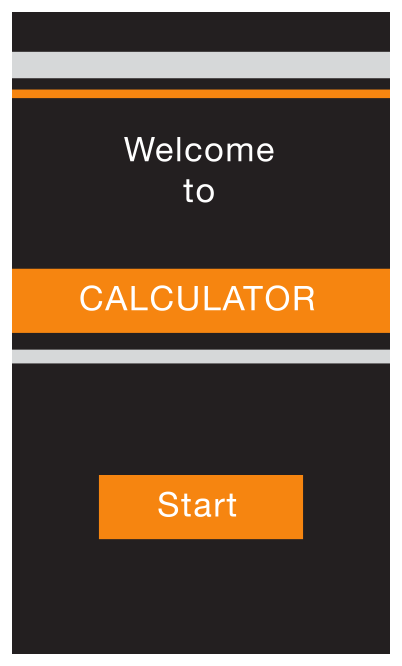
\includegraphics[width=4cm]{media/starting_2.png}
    \end{columns}
}

\frame{
    \frametitle{iOS: Navigation}
    \begin{itemize}
        \item iOS devices have no hardware `back button'
        \item Consider view hierarchy
        \begin{itemize}
            \item `Shallow' - many views accessible from one main view (e.g. Spotify: viewing playlists, profile, etc.)
            \item `Deep' - some long chains of views (e.g. eBay: creating a new auction)
        \end{itemize}
        \item Navigation usually handled by navigation bar   
        \item In general, try to only allow one path to each screen
    \end{itemize}
}

\frame{
    \frametitle{iOS: Modal contexts}
    \begin{itemize}
        \item Not recommended unless completely necessary:
        \begin{itemize}
            \item Critical to get user's attention
            \item A task must be completed or explicitly abandoned
        \end{itemize}
        \item Does not usually adhere to \alert{User control} principle as prevents further interaction
    \end{itemize}
}

\frame{
    \frametitle{iOS: Modal contexts}
    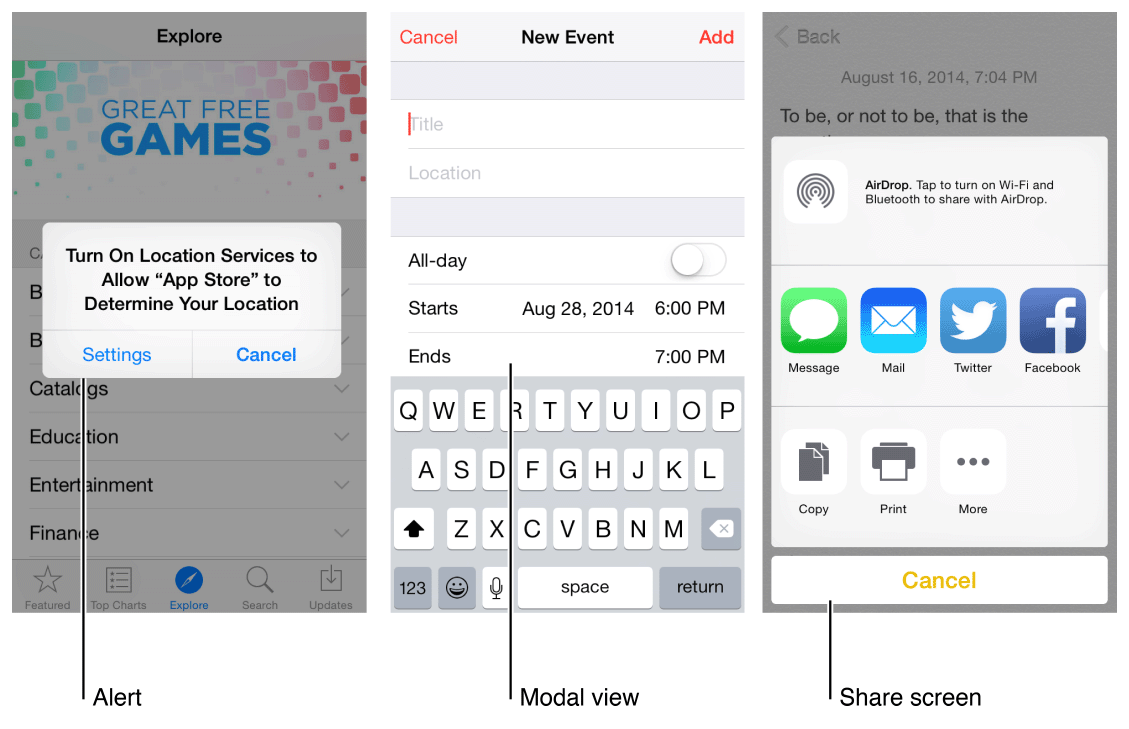
\includegraphics[width=\textwidth]{media/modal.png}
}

\frame{
    \frametitle{iOS: More guidelines...}
    \begin{itemize}
        \item Many more guidelines, including:
        \begin{itemize}
            \item Feedback (for aiding understanding \& Learnability)
            \item Animation (subtle animations make things more engaging and dynamic - Satisfaction)
            \item Colours, fonts, icons (indicate actions, behaviours, warnings, etc.)
            \item Terminology (use sensible words and common phrases to label actions and information
        \end{itemize}
        \item Provide really good guidelines for interface development in general
    \end{itemize}
}   

\frame{
    \frametitle{Designing for Android}
    Design guidelines: developer.android.com/design
    \vskip20pt
    \begin{columns}
        \column{.8\textwidth}
            \textbf{Creative vision:}
            \begin{itemize}
                \item \alert{Enchant me} - Fast, clear transitions, crisp layouts, beautiful icons
                \item \alert{Simplify my life} - Improve learnability, use simple tasks, let users feel in control
                \item \alert{Make me amazing} - Let people combine apps into new workflows
            \end{itemize}
            \vskip20pt
        \column{.2\textwidth}
            
\includegraphics[width=2cm]{media/android.jpg}
    \end{columns}        
}   

\frame{
    \frametitle{Android: Design principles}
    \begin{itemize}
        \item Delight me - careful animations, well-timed sounds, etc.
        \item Real objects more fun - allow interaction with objects within apps    
        \item Make it mine - let people add personal touches
        \item Keep it brief - short words and phrases
        \item Pictures are faster than words - use images/icons to portray actions/information
        \item Show things when I need them - make tasks small and menus relevant
        \item Only interrupt when important - shield people from irrelevant information
        \item Never user's fault - try and fix behind the scenes
        \item Make important things fast
    \end{itemize}
    \vskip10pt
    ... and more!
}

\frame{
    \frametitle{Android: Interface design}
    \begin{columns}
        \column{.5\textwidth}
            \begin{itemize}
                \item Google have incorporated most of their Android and web guidelines
                \item One design language across multiple platforms: Material Design
            \end{itemize}
        \column{.5\textwidth}
            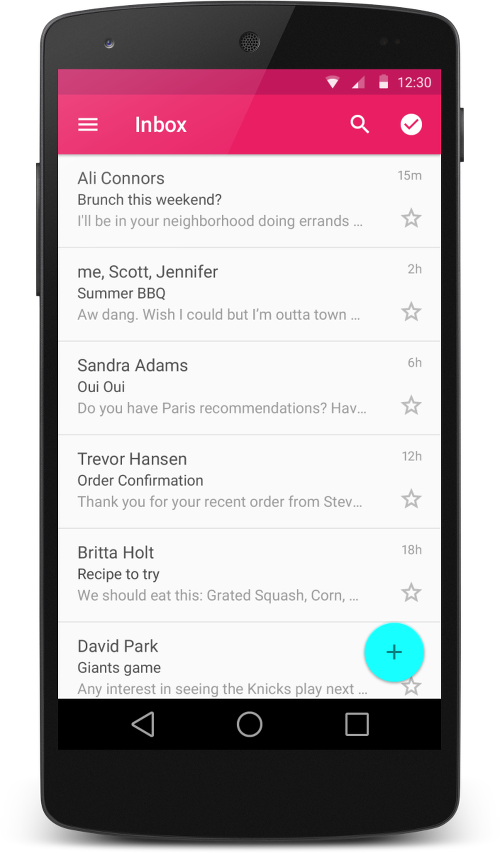
\includegraphics[width=4cm]{media/material_1.png}
    \end{columns}   
}

\frame{
    \frametitle{Google Material Design} 
    Design guidelines: google.com/design/spec/material-design
    \begin{itemize}
        \item Visual language
        \item Not necessarily platform-specific
        \item Designed for Android and the web
        \item Series of guidelines to help improve learnability and visibility
        \item Directly tie look and feel to action
    \end{itemize}
    \vskip20pt
}

\frame{
    \frametitle{Material Design: Principles}
    \begin{itemize}
        \item Material is metaphor - Make the display `feel' tactile
        \item Bold, graphic, intentional - Apply meaning and focus to components
        \item Motion provides meaning - Give motions to reinforce meaning behind actions
    \end{itemize}
    \vskip20pt
    Make the interface seem like it is made from material by providing depth, animation, and tactile features
}

\frame{
    \frametitle{Material Design: Basics}
    \begin{itemize} 
        \item Based around objects having 3D presence
        \item `Materials' have different sizes, but equal thickness
        \item Material casts shadows
        \item Material displays content, yet content doesn't add thickness
        \item Material is solid: events can't pass between layers and materials cannot move through eachother
    \end{itemize}   
}

\frame{
    \frametitle{Material Design: In general}
    \begin{itemize}
        \item Objects occupy 3D space
        \item Material has \alert{elevation}
        \item Therefore has \alert{shadow}
        \item Similar material (e.g. colours, shapes) should have similar \alert{functions} or \alert{purposes}
        \item Material has mass, so \alert{animate} accordingly
        \item Material should acknowledge interaction
    \end{itemize}
    \vskip10pt
    Many more  guidelines...\\
    \textbf{Check out: material-ui.com}
}

\frame{
    \frametitle{In general...}
    \begin{itemize}
        \item Although guidelines are platform-specific, most are useful in general case too
        \item You \textbf{won't} be examined on any platform-specific design guidelines
        \item Useful to see how official guidelines link to theory we've covered in lectures
        \item They provide useful examples of how usability principles can be adhered to
        \item Useful to know where to find guidance on good interface design
    \end{itemize}
    \vskip20pt
    Guidelines for popular platforms are often useful in general too.
}

\frame{
    \frametitle{Summary}
    \begin{itemize}
        \item Advantages and disadvantages of platform-specific design
        \item iOS human interface guidelines
        \item Android design guidelines
        \item Material Design
    \end{itemize}
}    

\end{document}
